\documentclass{article}
\usepackage[margin=2cm]{geometry}
\usepackage{graphicx}
\usepackage{hyperref}

\title{Snake: Developer Guide}
\author{Alessandra Sasanelli, Simone Maccario}
\date{\today}

\begin{document}
	\maketitle
	\abstract{
		This document is meant to show the source code of the project. 
		After giving a brief overview on the structure of the project, the libraries used and how are the code is divided between the files, 
		it will illustrate all of the main functions.
	}
	
	\section{The structure of the project}
	The folder of the main project contains 3 subdirectories: 
	\begin{itemize}
		\item docs is meant to hold all of the non-relevant to code files, like the README.txt, the proposal and the two guides
		\item resources is used to hold all of the images and sounds used by the game: into the images folder there are all of the images; into the sounds folder there are all of the sounds, whilst in the numbers folder, there are the images of the numbers (used to track the user score)
		\item code holds all of the source files for the project; inside, the subdirectory external-files has all of the auxiliary code files
	\end{itemize}
	
	\section{The libraries}	
	This project uses three main libraries:
	\begin{itemize}
		\item \textbf{racket/base} --$>$ used to import and export functions, structures and constants from file to file 
		(\href{https://docs.racket-lang.org/reference/index.html}{documentation})
		\item \textbf{2htdp/universe} --$>$ used to make the interactive application thanks to the provided big-bang function 
		(\href{https://docs.racket-lang.org/teachpack/2htdpuniverse.html}{documentation})
		\item \textbf{2htdp/image} --$>$ used to render the application. From this library, we imported also racket/gui/base play-sound (\href{https://docs.racket-lang.org/gui/Windowing_Functions.html#\%28def._\%28\%28lib._mred\%2Fmain..rkt\%29._play-sound\%29\%29}{documentation of the function here}) function 	
		(\href{https://docs.racket-lang.org/teachpack/2htdpimage.html}{documentation})
	\end{itemize}
	
	\pagebreak
	
	\section{Source code}
	This section will discuss the main functions developed to make the application. It will focus on every single file to explain the functions present in each of them.
	
	\subsection{positions.rkt}
	This file contains all the functions relative to the positions; below, are listed and explained a few of them.
	Here won't be listed all simple auxiliary functions, which are: increment-pos, decrement-pos, direction-by-posn, delete-el.
	\begin{itemize}
		\item \textbf{make-positions}: \\
			\emph{signature}: Number Number Number List$<$Posn$>$ -$>$ List$<$Posn$>$ \\
			\emph{purpose}: computes all the positions on the background before the game starts \\
			\emph{explanation}: this function takes in 4 inputs. The first one, n, represents the positions from which we are starting to compute all of the other positions, x and y represents the row and column from which we are starting, then the list represents a list with all the positions already present. To compute all the positions for a background with 501*501 dimensions, and, considering that every position takes 25*25 pixels of area, you must insert pass as parameters 1, 1, 1 (list (make-posn 13 13)), and this recursion must stop at 400, which is the max number of positions available, given the background dimensions. This is why the base case for this function is when n is equal to 400. For every other case, we first check whether the row has all been filled up; this means that we need to increment n and to change row, incrementing y by one. Otherwise, we need to increment n by one and x by one to change column. The posn will be created based on the column and the row and it will be added to the list of positions.
			\begin{figure}[h!]
				\centering
				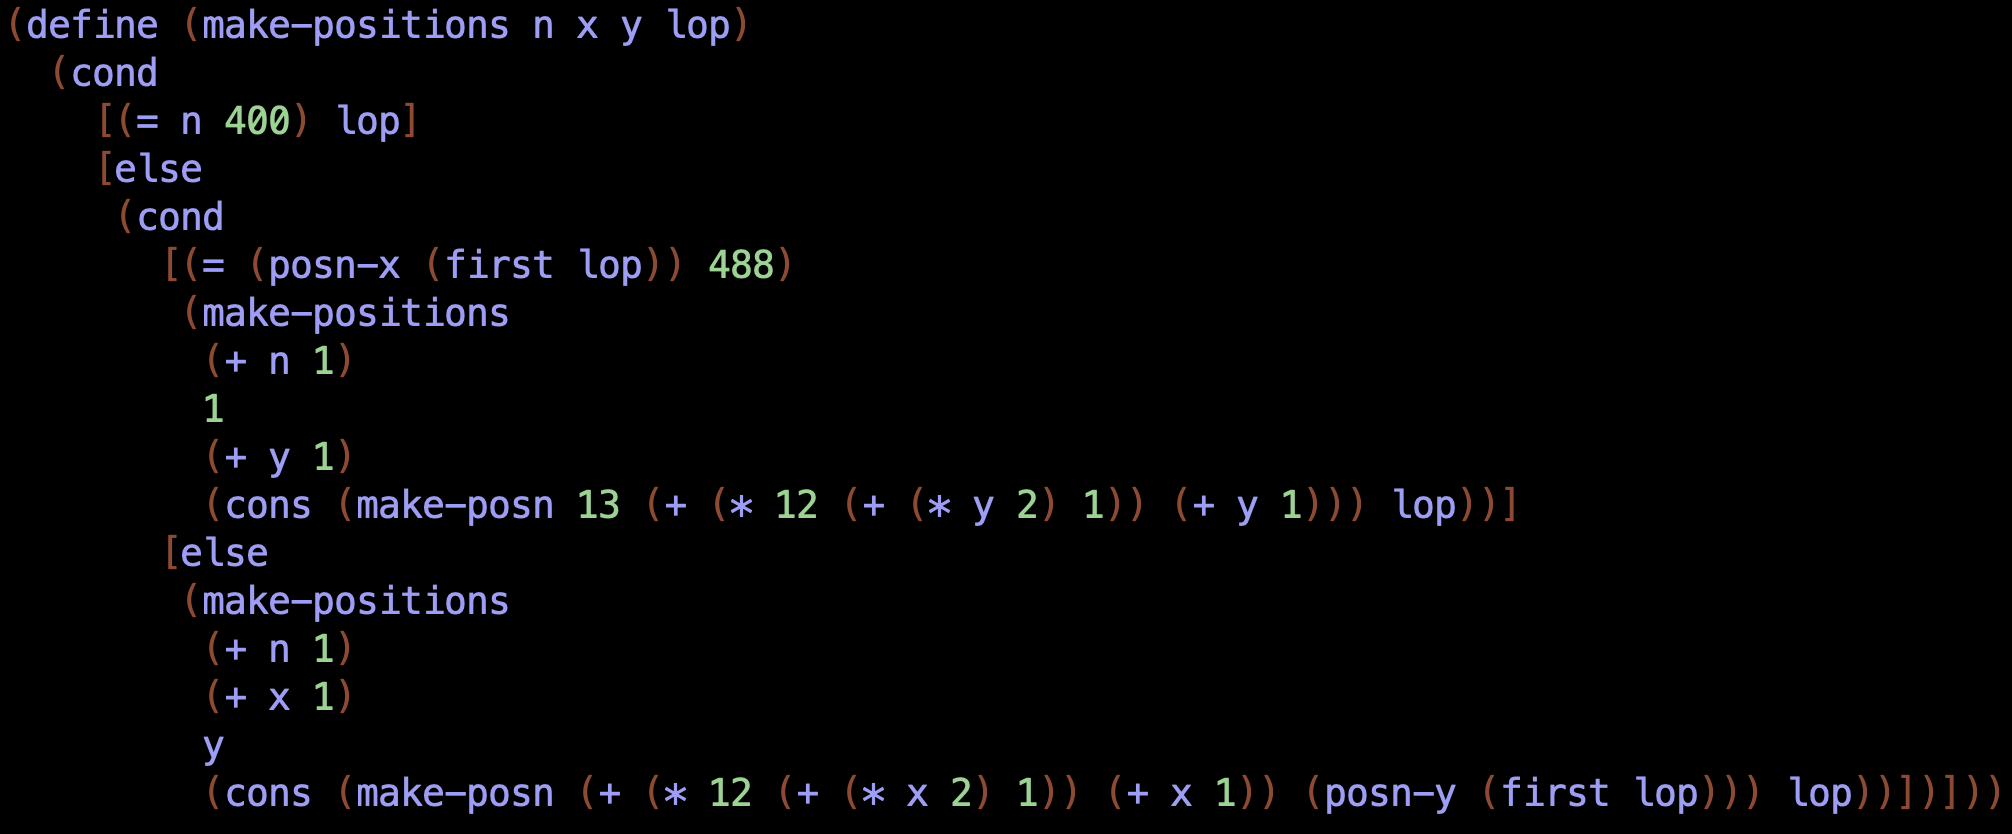
\includegraphics[width=.6\linewidth]{make-position.png}
				\caption{make-position function in racket}
			\end{figure}
			
		\item \textbf{compute-available-pos}: \\
			\emph{signature}: List$<$Posn$>$ List$<$Posn$>$ -$>$ List$<$Posn$>$ \\
			\emph{purpose}: computes available positions on the background \\
			\emph{explanation}: this function needs to do recursion over two lists, the lop-snake which represents the positions of the snake 							to be eliminated from the available positions, the lop list. The base case checks whether one or both of the 							two lists are empty. In this case, all the positions have been checked and none of them is occupied, 									therefore, we return lop. Else, we call the function on the rest of the lop-snake and delete-el over the first of 							the lop-snake and on the lop function. This function returns either lop as it is, or it eliminates one element 								from it if it is equal to first of lop-snake. 
			\begin{figure}[h!]
				\centering
				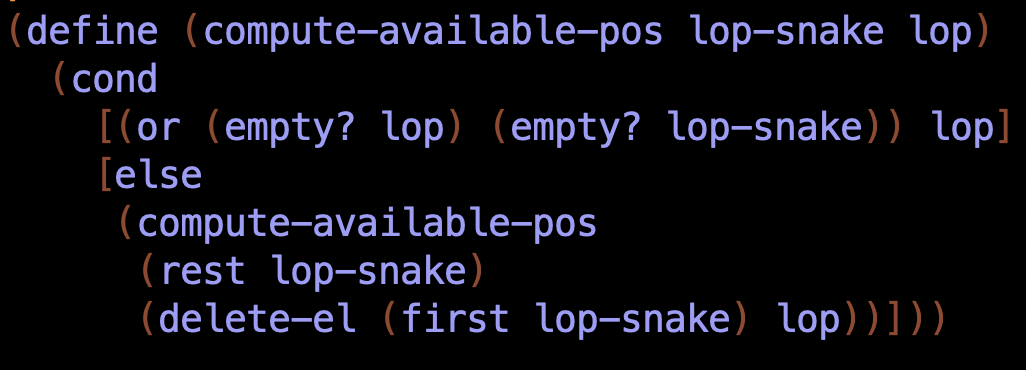
\includegraphics[width=.6\linewidth]{compute-available-pos.png}
				\caption{compute-available-pos function in racket}
			\end{figure}
			
		\item \textbf{compute-apple-position}: \\
			\emph{signature}: Number Number List$<$Posn$>$ -$>$ Apple \\
			\emph{purpose}: computes all the positions on the background before the game starts \\
			\emph{explanation}: this function uses three parameters, one of which is an accumulator. The n represent a number which must be between 1(included) and 401(excluded). This number represent which position from the available positions to choose. The base case checks if the rest is empty or if the n is equal to the accumulator (which means that ). This condition returns the first element. Else, we call recursively the function over the rest of the list and we increase by one the accumulator. 
			\begin{figure}[h!]
				\centering
				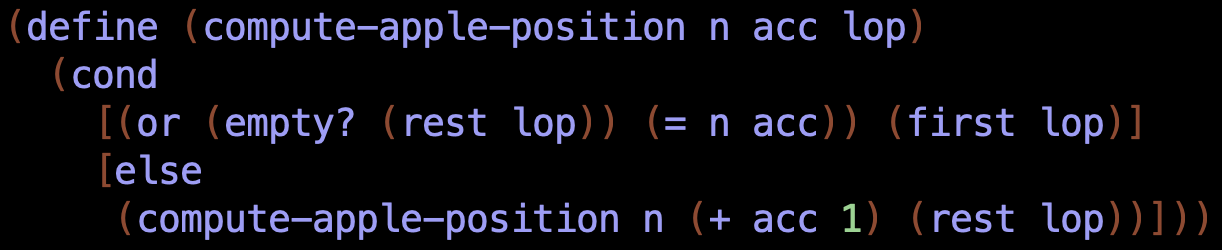
\includegraphics[width=.6\linewidth]{compute-apple-position.png}
				\caption{compute-apple-position function in racket}
			\end{figure}
			
		\item \textbf{check-position-out}: \\
			\emph{signature}: Posn List$<$Posn$>$ -$>$ Boolean \\
			\emph{purpose}: checks wheather the given posn is into backgroundpos \\
			\emph{explanation}: in the base case, if the list is empty, the list returns true. 
							The other case happens if the first element of the list is equal to pos; at this point, the function returns 								false.
							In the recursive case, we simply call the function again on the rest of the list.
			\begin{figure}[h!]
				\centering
				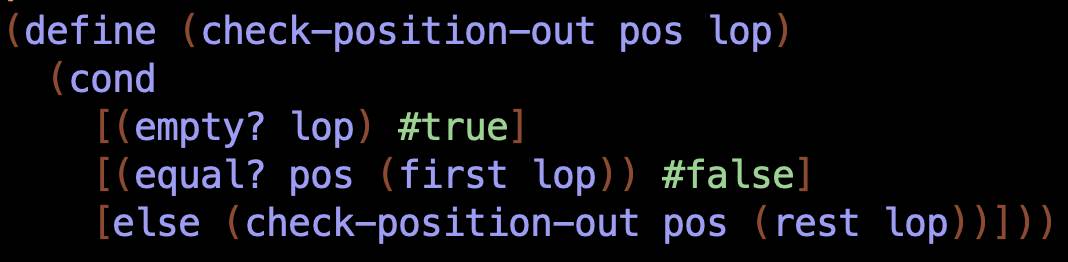
\includegraphics[width=.6\linewidth]{check-position-out.png}
				\caption{check-position-out function in racket}
			\end{figure}
			
		\item \textbf{update-positions}: \\
			\emph{signature}: Direction List$<$Posn$>$ -$>$ List$<$Posn$>$ \\
			\emph{purpose}: updates a list of positions based on itself and the head direction \\
			\emph{explanation}: this function takes a list of posn and returns a new list of posn. The new posn will be updated based on a 							direction. 
							The base case for this function happens when the rest of the list is empty. This means that the only 									element that the only posn that is left to be updated is the head. This posn will follow the direction field 								given in the snake struct. The recursive case constructs a list applying to the first element of the list the 								function "compute-new-posn", wich simply returns a new posn based on the direction passed to the 									function. The direction for a single posn is given by itself and the next posn present into the list.
			\begin{figure}[h!]
				\centering
				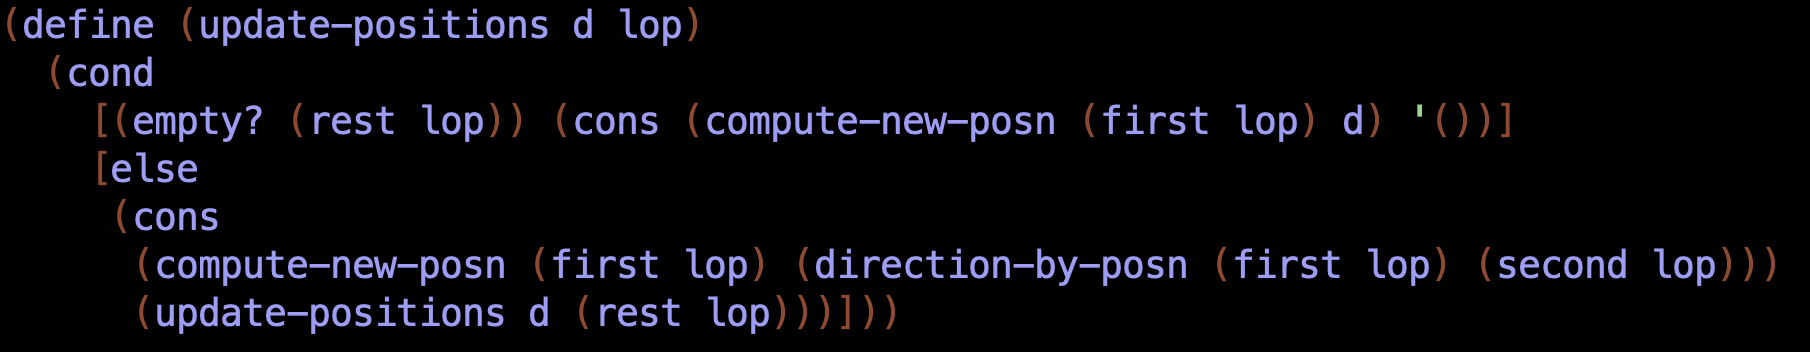
\includegraphics[width=.6\linewidth]{update-positions.png}
				\caption{update-positions function in racket}
			\end{figure}
	\end{itemize}
	
	\pagebreak
	
	\subsection{snake.rkt}
	This file contains all the functions relative to the snake. Of all the functions written, it is only shown the main one, the draw-snake. The others are: change-snake-direction, which simply returns a snake with changed direction based on the direction inputed, move-snake which return a snake but calling the update-positions on the snake-position, check-eat-snake which simply returns true if the position of the head is equal to any other into the snake-position.
	\begin{itemize}
		\item \textbf{draw-snake}: \\
			\emph{signature}: Snake -$>$ Image \\
			\emph{purpose}: draws the snake on the background \\
			\emph{explanation}: since the snake is graphically made of three basic elements, which are the head, the tail and the snakeunit, we need three conditions to be applied in our recursion. The base case happens when the rest of the list is empty; this means that the only element to be drawn is the head of the snake, so, we place the head over the background at the position specified. The head needs also to be rotated based on its direction, that's why we call rotate-el on it. Then, the second condition happens when the length of the list is equal to the length of the snake; this means that the element to be drawn is the tail of the snake. Rotate-el is applied to the tail too, but the direction of the tail is now given by itself and the next element after it. The recursive case calls the place-image on the first element of the list, drawing a snakeunit at specified position over the result of the recursive call applied to the rest of the list.  
			\begin{figure}[h!]
				\centering
				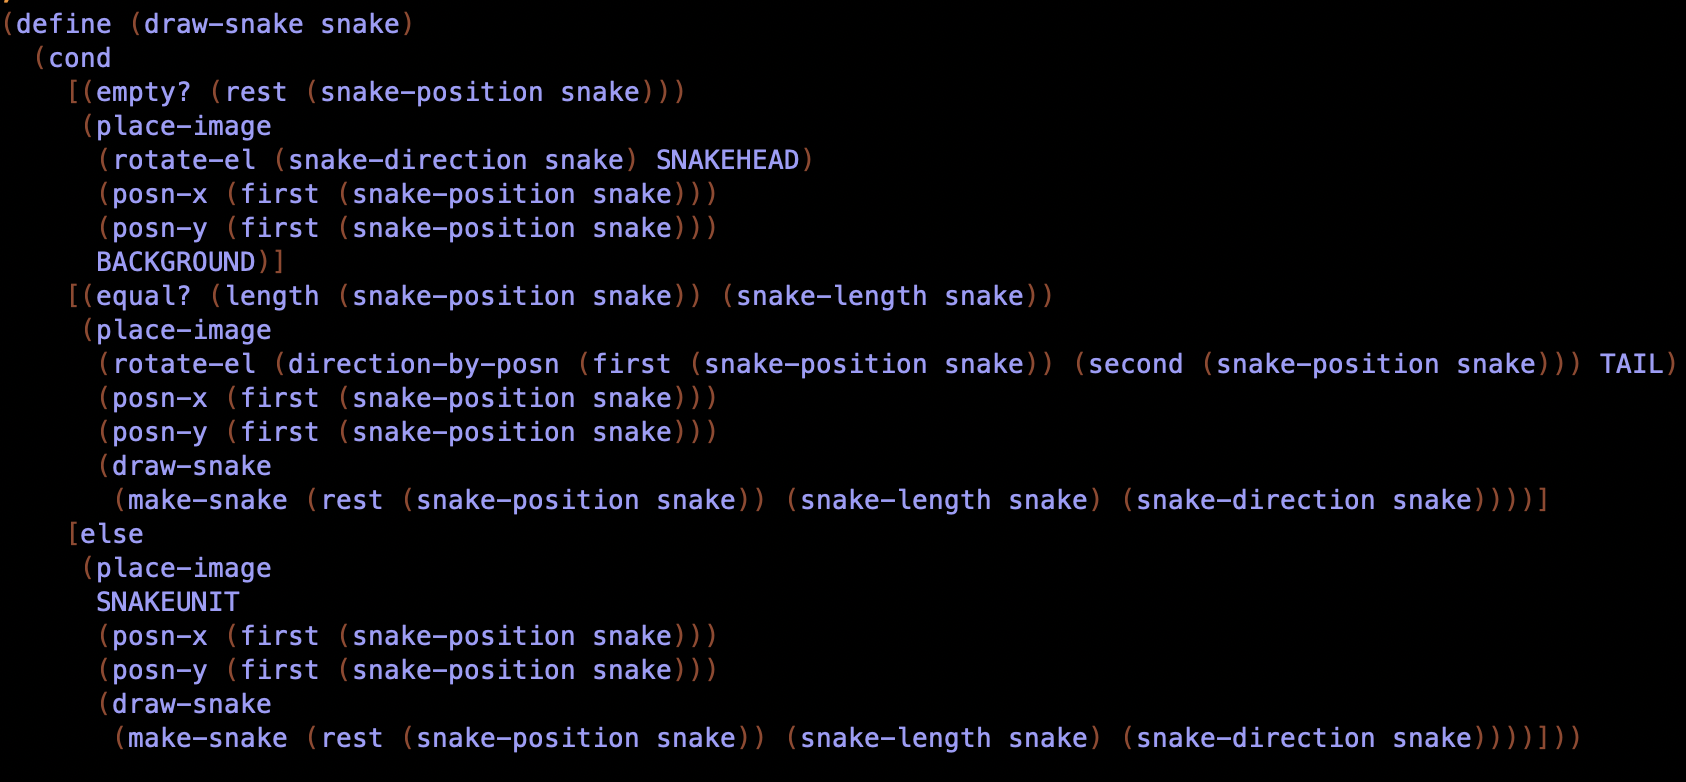
\includegraphics[width=.6\linewidth]{draw-snake.png}
				\caption{draw-snake function in racket}
			\end{figure}
	\end{itemize}
	
	\subsection{generals.rkt}
	This file contains all the functions that are of general purpose. This file mainly provides constants, but it also provides two functions, one of which will be explained here. One important constant is the NUMBERS, which is a list containing the paths to the images of the single numbers.
	\begin{itemize}
		\item \textbf{number-$>$image}: \\
			\emph{signature}: StringOfNumbers Number -$>$ Image \\
			\emph{purpose}: takes in a number and returns it as an image \\
			\emph{explanation}: the number n represents the initial indices of the character in the string of numbers. So, the base case will be when n-1 is equal to the string length. In this case, we just call the bitmap/file function on the path of the file, which gets returned by the function number-$>$path. The recursive case simply calls the beside function on the element of the string at index n and on the recursive call on the function with the same string and n incremented by one.
			\begin{figure}[h!]
				\centering
				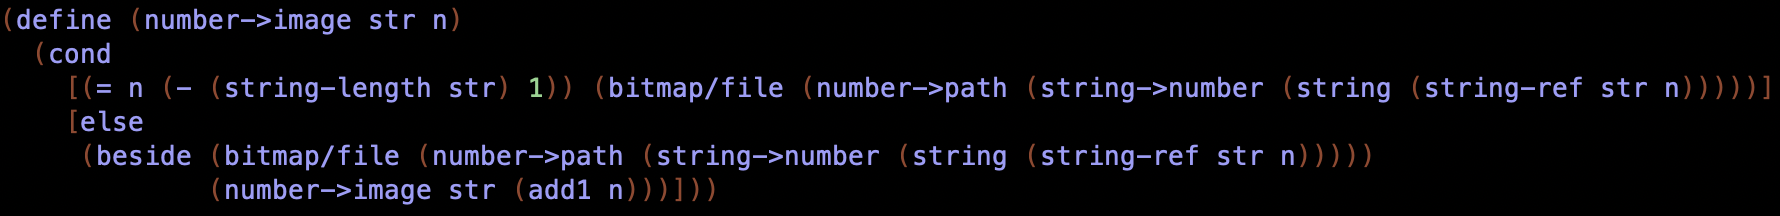
\includegraphics[width=.6\linewidth]{number-image.png}
				\caption{number-image function in racket}
			\end{figure}
	\end{itemize}
	
	\pagebreak
	
	\subsection{snake-final.rkt}
	This file contains all the functions that are needed to make the big-bang work. Most of these functions take in an Appstate.
	\begin{itemize}
		\item \textbf{handle-keyboard}: \\
			\emph{signature}: AppState KeyboardEvent -$>$ AppState \\
			\emph{purpose}: handles the keyboard events \\
			\emph{explanation}: this function is a big conditional that checks the string KeyboardEvent. If the key pressed is "s", then we call the start function, which simply sets the game field to true. The second condition check if the key arrow pressed is opposite to the direction the snake head had previously to block the operation. If "r" is pressed, the function calls the reset function, which simply returns the default appstate. The "escape" key changes the quit field to true, making the app quitting and closing right after. For every other case, the function simply returns the given state.
			\begin{figure}[h!]
				\centering
				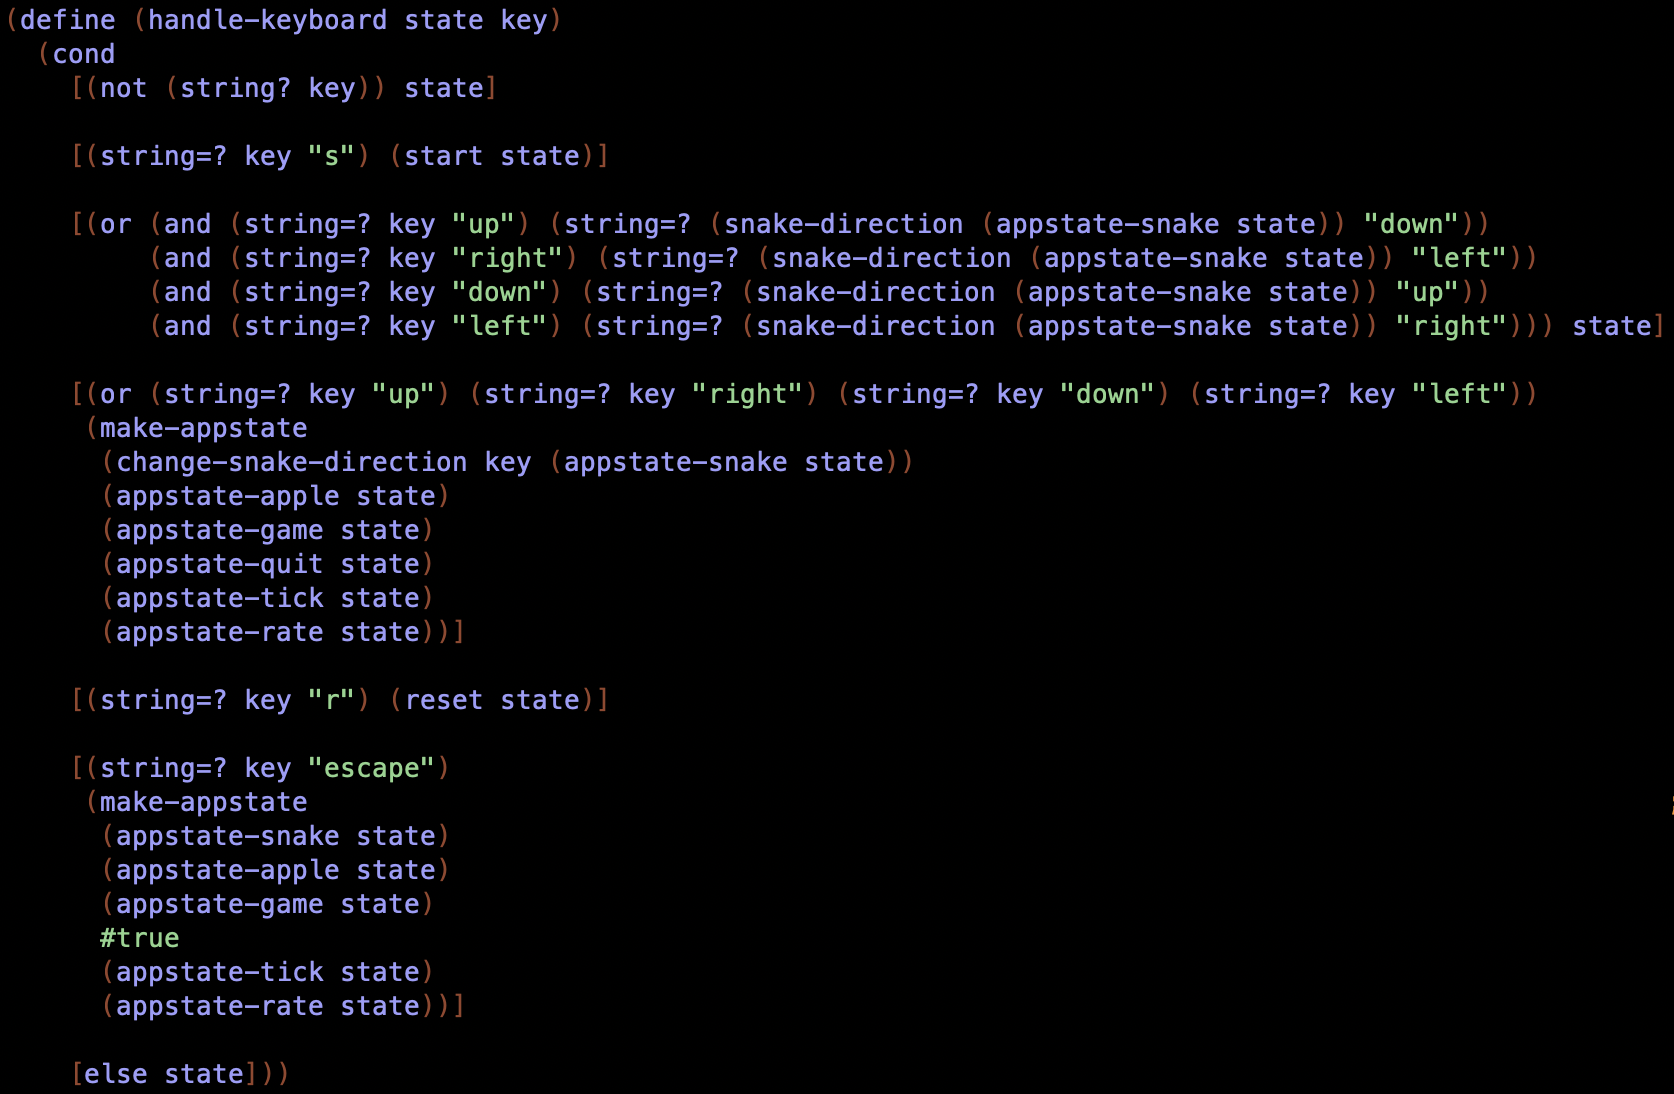
\includegraphics[width=.6\linewidth]{handle-keyboard.png}
				\caption{handle-keyboard function in racket}
			\end{figure}
			
		\item \textbf{eating}: \\
			\emph{signature}: AppState -$>$ AppState \\
			\emph{purpose}: handles the eating event of the game \\
			\emph{explanation}: the first operation the function does, is playing the sound when it gets called. Then, it comes the main part of the function: an appstate gets created with a new snake on which gets called the before described move-snake. This snake, though, has a new position added to the snake-position field, and the length gets incremented by one. Then, the apple changes; its position gets computed by the compute-apple-pos, passing a list containing the snake positions and the previous apple position, and all the positions on the background. The last field that is different from before is the rate field, which gets decremented by one only if three apples have been eaten.
			\begin{figure}[h!]
				\centering
				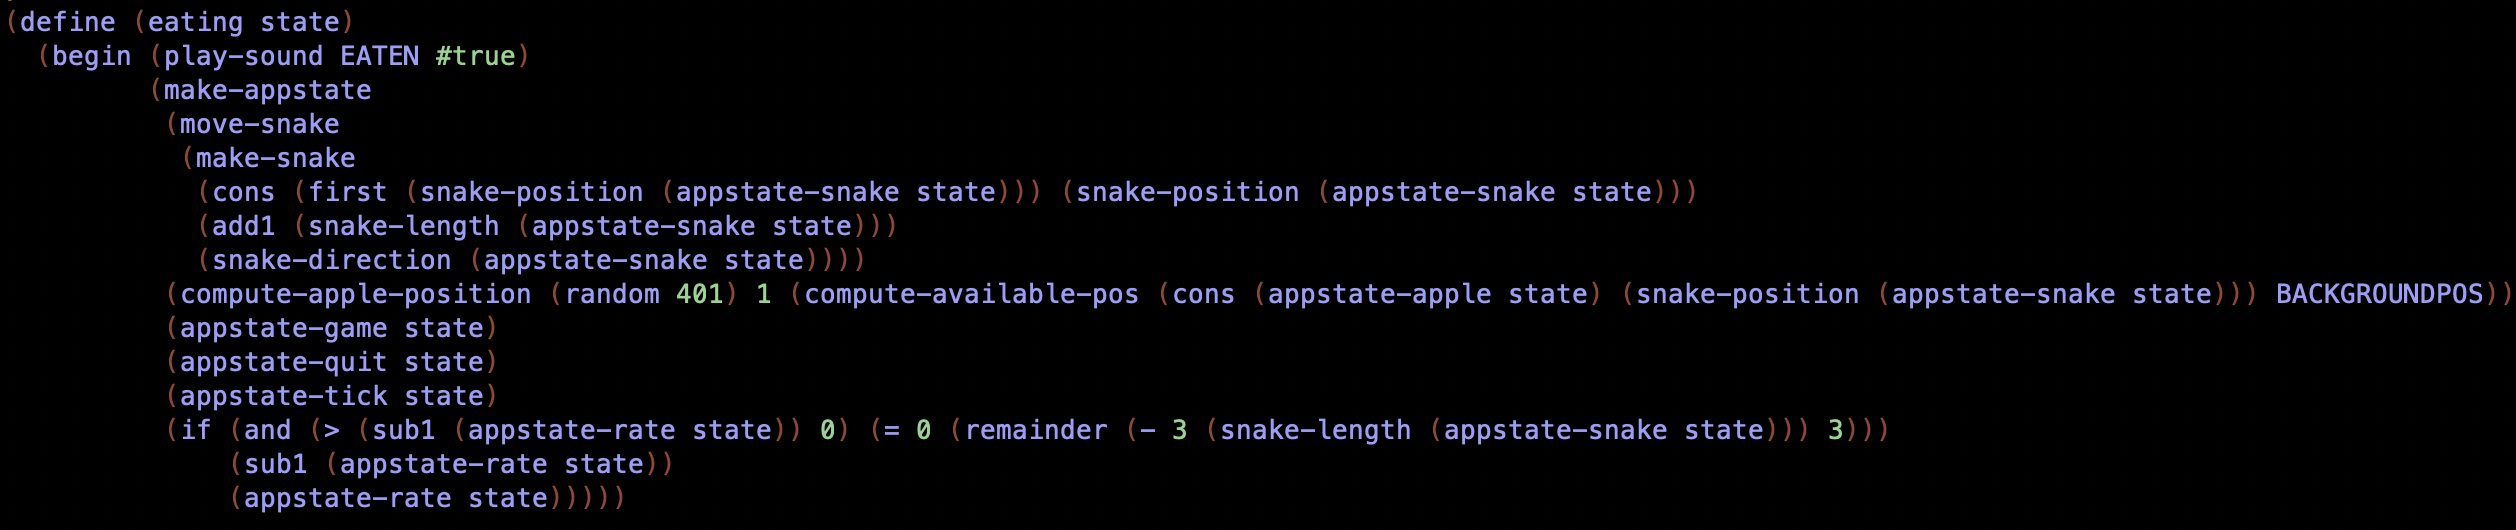
\includegraphics[width=.6\linewidth]{eating.png}
				\caption{eating function in racket}
			\end{figure}
			
		\item \textbf{move}: \\
			\emph{signature}: AppState -$>$ AppState \\
			\emph{purpose}: used to change the appstate on tick \\
			\emph{explanation}: if on tick, it results that the end condition is meet, the game and quit fields get switched to false. Then, if the appstate game is false, the function simply returns the same appstate as before. Then, we check for the remainder between tick and rate. Tick represents the number of times the clock ticked from the beginning, while the rate represents the speed levels. If the remainder is zero, we update the appstate, either by simply calling move-snake on the snake, or by calling the eating function. Thanks to this method, as the rate gets smaller, the snake gets faster. If none of the conditions named before are not met, the appstate gets returned as before but incrementing by one the tick field.
			\begin{figure}[h!]
				\centering
				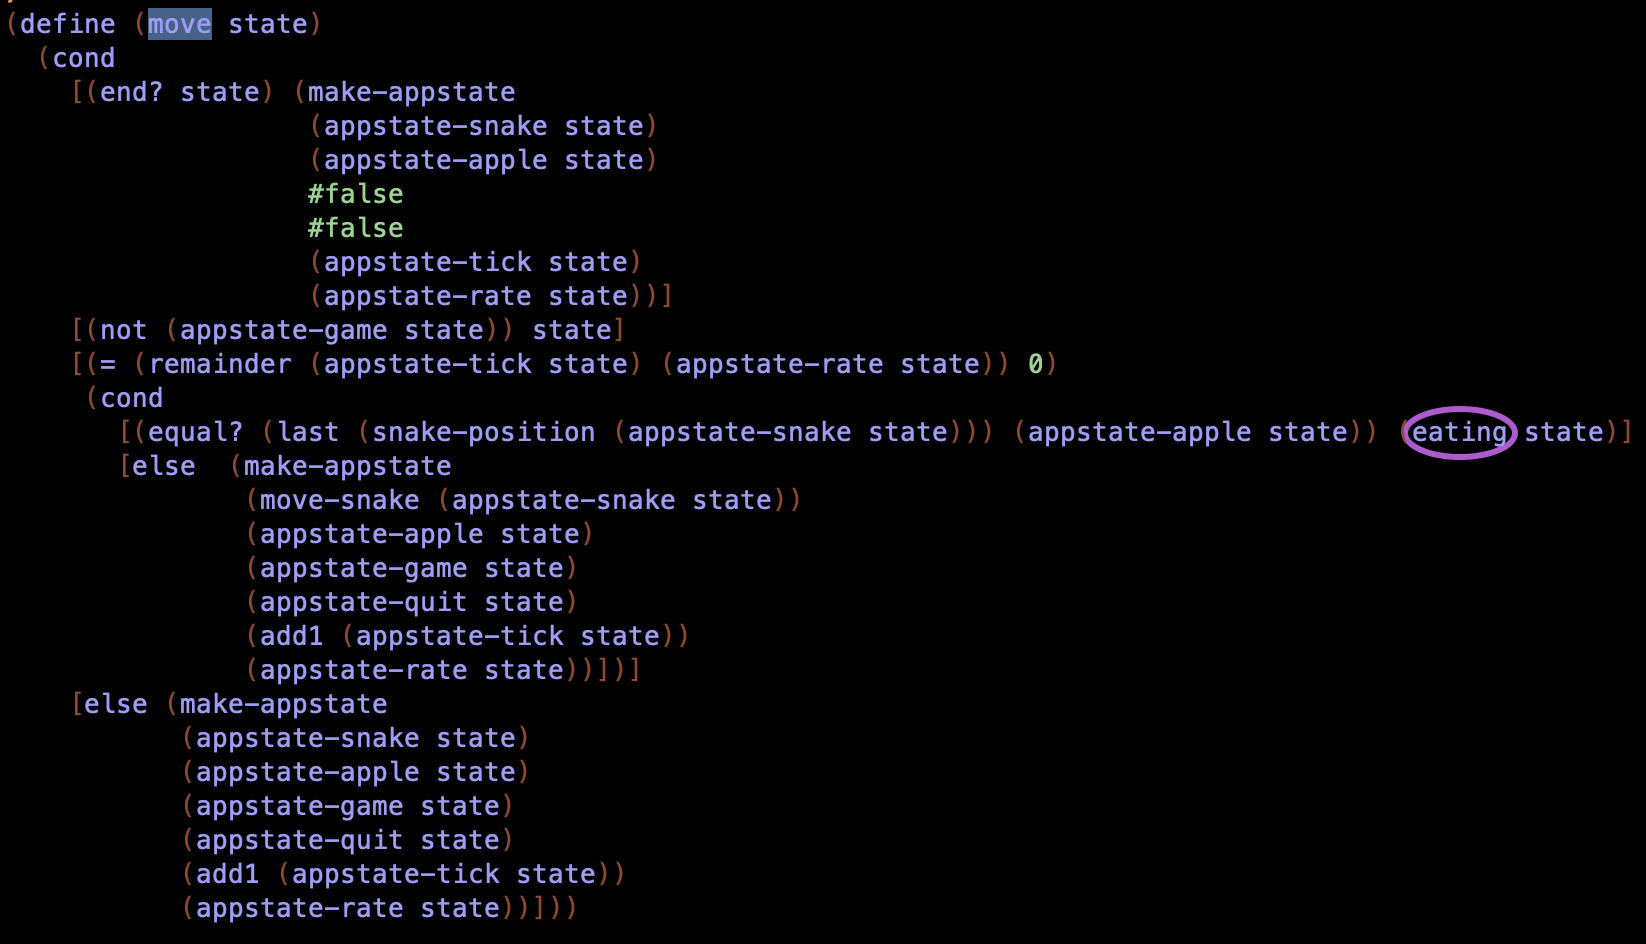
\includegraphics[width=.6\linewidth]{move.png}
				\caption{move function in racket}
			\end{figure}
			
		\item \textbf{end?}: \\
			\emph{signature}: AppState -$>$ Boolean \\
			\emph{purpose}: checks weather the game is in gameover or not \\
			\emph{explanation}: it simply checks whether the snake has gone over the borders of the game or if it has eaten itself. Then, if this condition is true, the function returns true and plays the game over sound, setting the GAMEOVRPLAYED to true. Otherwise, it resets GAMAOVRPLAYED to false and return false.
			\begin{figure}[h!]
				\centering
				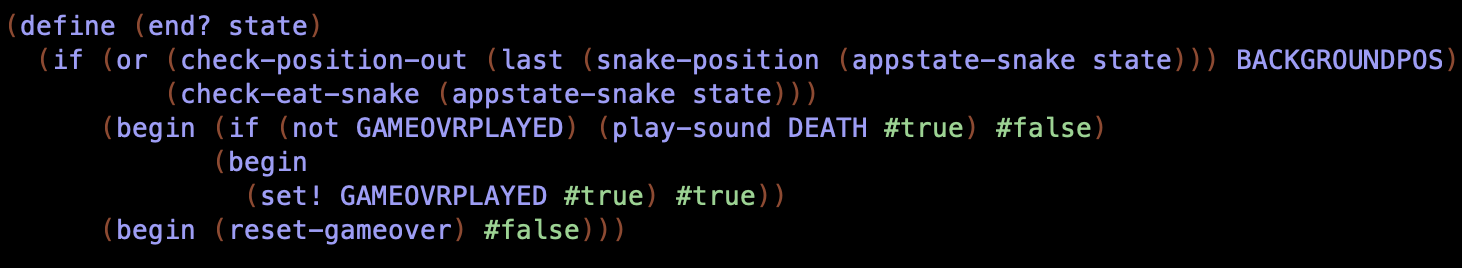
\includegraphics[width=.6\linewidth]{end.png}
				\caption{end? function in racket}
			\end{figure}
	\end{itemize}

\end{document}